\section*{Problem 2: Tries}


\noindent
\textbf{a)} Zeichnen Sie einen unkomprimierten und einen komprimierten Trie für die Wörter \{ALGORITHMUS, TRIE, BAUM, TORUS, BAHN, TORPEDO\}.\\



\textbf{Aufgabe 2a:} 
\textbf{unkomprimierter Trie:}
\begin{center}
    \textbf{1. insert(ALGORITHMUS)}
\end{center}
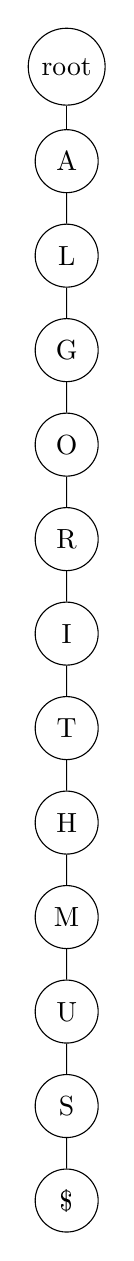
\begin{tikzpicture}[
  level distance=1.2cm,
  every node/.style={draw, circle, minimum size=0.8cm}
]


\node {root}
  child {node {A}
    child {node {L}
      child {node {G}
        child {node {O}
          child {node {R}
            child {node {I}
              child {node {T}
                child {node {H}
                  child {node {M}
                    child {node {U}
                      child {node {S}
                        child {node {\$}}
                      }
                    }
                  }
                }
              }
            }
          }
        }
      }
    }
  };
\end{tikzpicture}

\newpage

\begin{center}
    \textbf{2. insert(TRIE)}
\end{center}
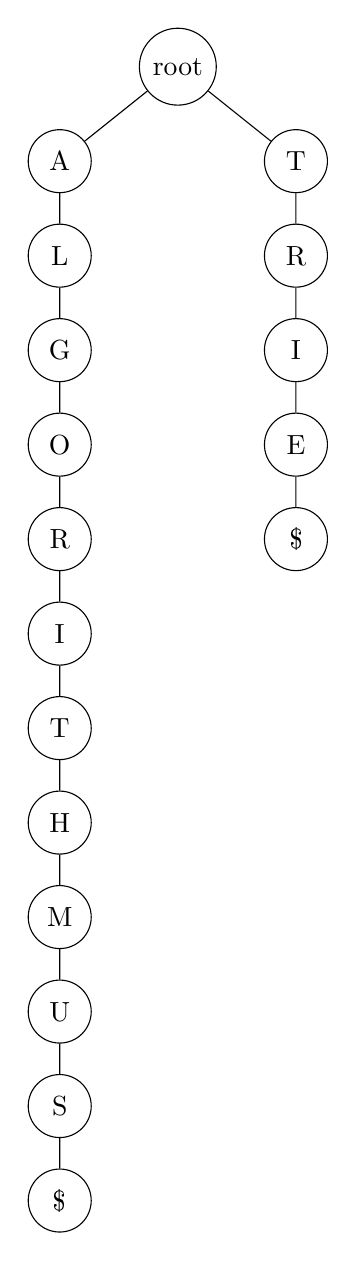
\begin{tikzpicture}[
  level distance=1.2cm,
  level 1/.style={sibling distance=3cm},
  every node/.style={draw, circle, minimum size=0.8cm}
]

\node {root}
  child {node {A}
    child {node {L}
      child {node {G}
        child {node {O}
          child {node {R}
            child {node {I}
              child {node {T}
                child {node {H}
                  child {node {M}
                    child {node {U}
                      child {node {S}
                        child {node {\$}}
                      }
                    }
                  }
                }
              }
            }
          }
        }
      }
    }
  }
  child {node {T}
    child {node {R}
      child {node {I}
        child {node {E}
          child {node {\$}}
        }
      }
    }
  };
\end{tikzpicture}

\newpage

\begin{center}
    \textbf{3. insert(BAUM)}
\end{center}
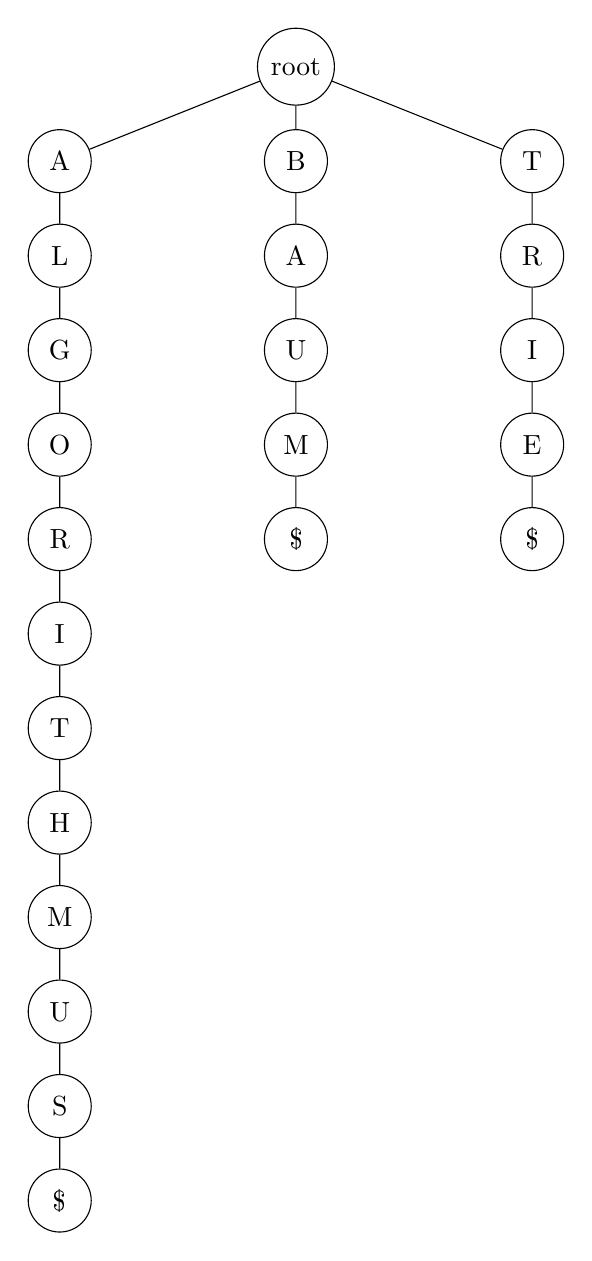
\begin{tikzpicture}[
  level distance=1.2cm,
  level 1/.style={sibling distance=3cm},
  level 2/.style={sibling distance=1.5cm},
  every node/.style={draw, circle, minimum size=0.8cm}
]

\node {root}
  child {node {A}
    child {node {L}
      child {node {G}
        child {node {O}
          child {node {R}
            child {node {I}
              child {node {T}
                child {node {H}
                  child {node {M}
                    child {node {U}
                      child {node {S}
                        child {node {\$}}
                      }
                    }
                  }
                }
              }
            }
          }
        }
      }
    }
  }
  child {node {B}
    child {node {A}
      child {node {U}
        child {node {M}
          child {node {\$}}
        }
      }
    }
  }
  child {node {T}
    child {node {R}
      child {node {I}
        child {node {E}
          child {node {\$}}
        }
      }
    }
  };
\end{tikzpicture}

\newpage

\begin{center}
    \textbf{4. insert(TORUS)}
\end{center}
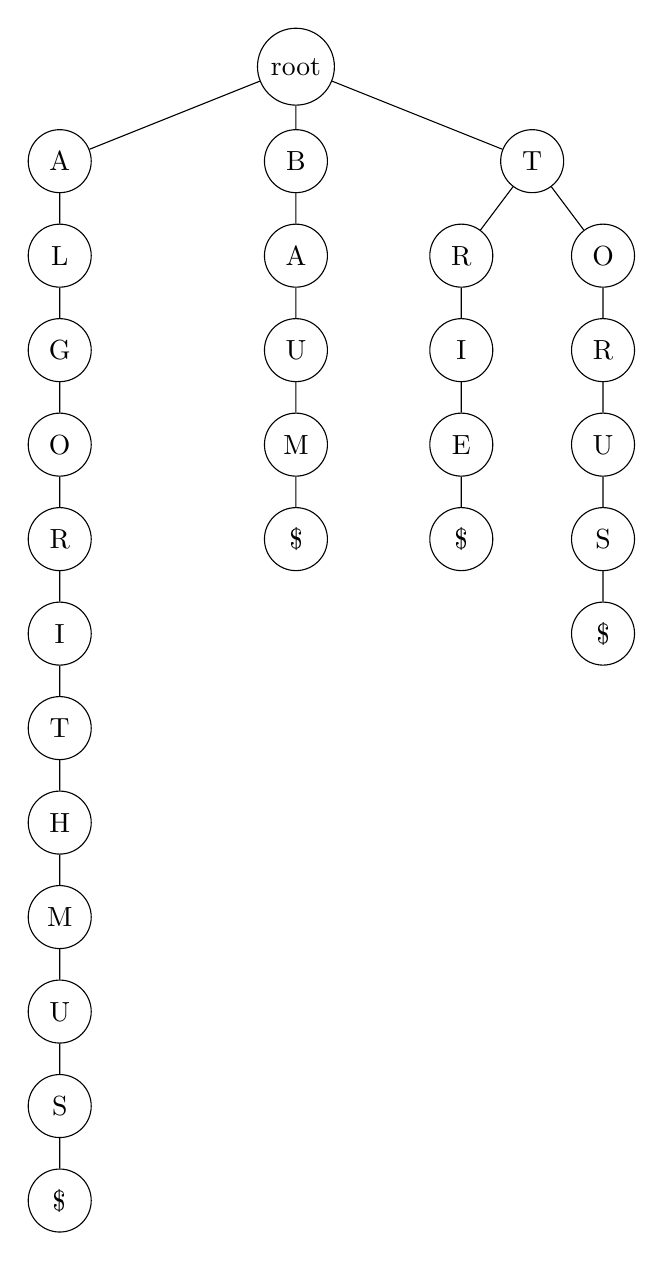
\begin{tikzpicture}[
  level distance=1.2cm,
  level 1/.style={sibling distance=3cm},
  level 2/.style={sibling distance=1.8cm},
  level 3/.style={sibling distance=1.5cm},
  every node/.style={draw, circle, minimum size=0.8cm}
]

\node {root}
  child {node {A}
    child {node {L}
      child {node {G}
        child {node {O}
          child {node {R}
            child {node {I}
              child {node {T}
                child {node {H}
                  child {node {M}
                    child {node {U}
                      child {node {S}
                        child {node {\$}}
                      }
                    }
                  }
                }
              }
            }
          }
        }
      }
    }
  }
  child {node {B}
    child {node {A}
      child {node {U}
        child {node {M}
          child {node {\$}}
        }
      }
    }
  }
  child {node {T}
    child {node {R}
      child {node {I}
        child {node {E}
          child {node {\$}}
        }
      }
    }
    child {node {O}
      child {node {R}
        child {node {U}
          child {node {S}
            child {node {\$}}
          }
        }
      }
    }
  };
\end{tikzpicture}

\newpage

\begin{center}
    \textbf{5. insert(BAHN)}
\end{center}
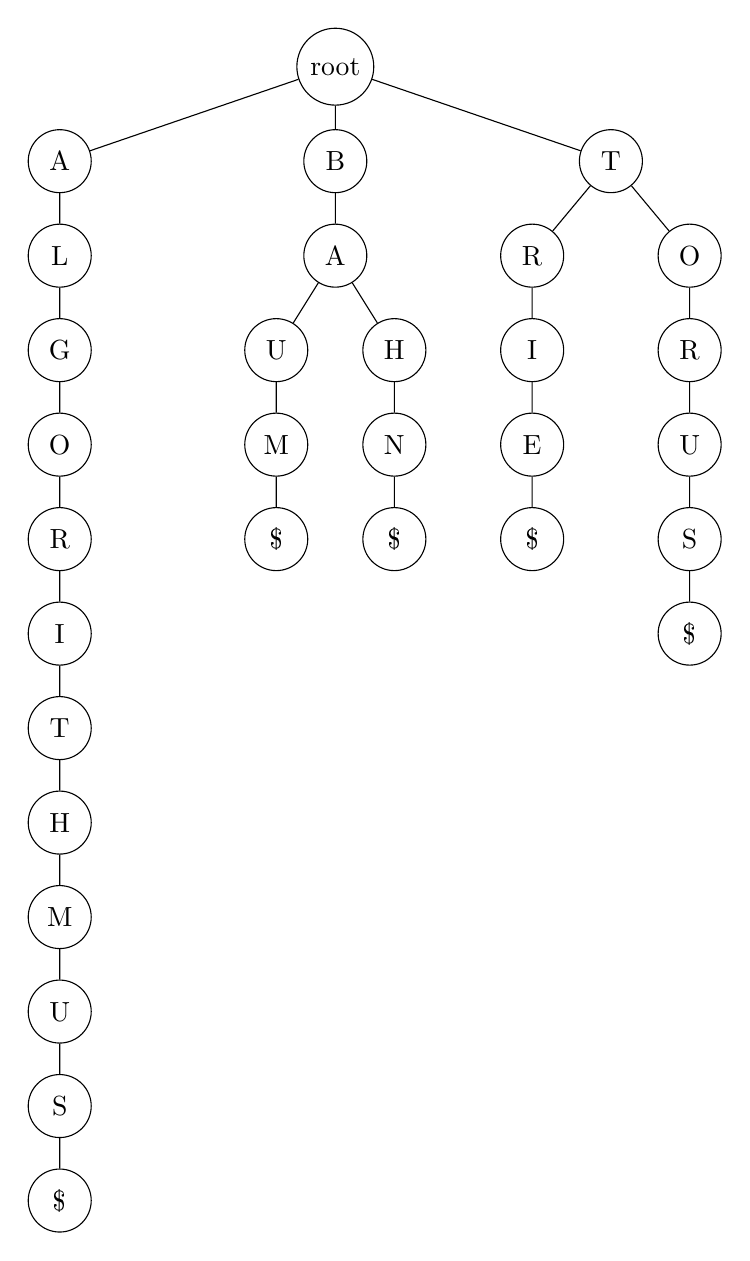
\begin{tikzpicture}[
  level distance=1.2cm,
  level 1/.style={sibling distance=3.5cm},
  level 2/.style={sibling distance=2cm},
  level 3/.style={sibling distance=1.5cm},
  every node/.style={draw, circle, minimum size=0.8cm}
]

\node {root}
  child {node {A}
    child {node {L}
      child {node {G}
        child {node {O}
          child {node {R}
            child {node {I}
              child {node {T}
                child {node {H}
                  child {node {M}
                    child {node {U}
                      child {node {S}
                        child {node {\$}}
                      }
                    }
                  }
                }
              }
            }
          }
        }
      }
    }
  }
  child {node {B}
    child {node {A}
      child {node {U}
        child {node {M}
          child {node {\$}}
        }
      }
      child {node {H}
        child {node {N}
          child {node {\$}}
        }
      }
    }
  }
  child {node {T}
    child {node {R}
      child {node {I}
        child {node {E}
          child {node {\$}}
        }
      }
    }
    child {node {O}
      child {node {R}
        child {node {U}
          child {node {S}
            child {node {\$}}
          }
        }
      }
    }
  };
\end{tikzpicture}

\newpage

\begin{center}
    \textbf{6. insert(TORPEDO)}
\end{center}
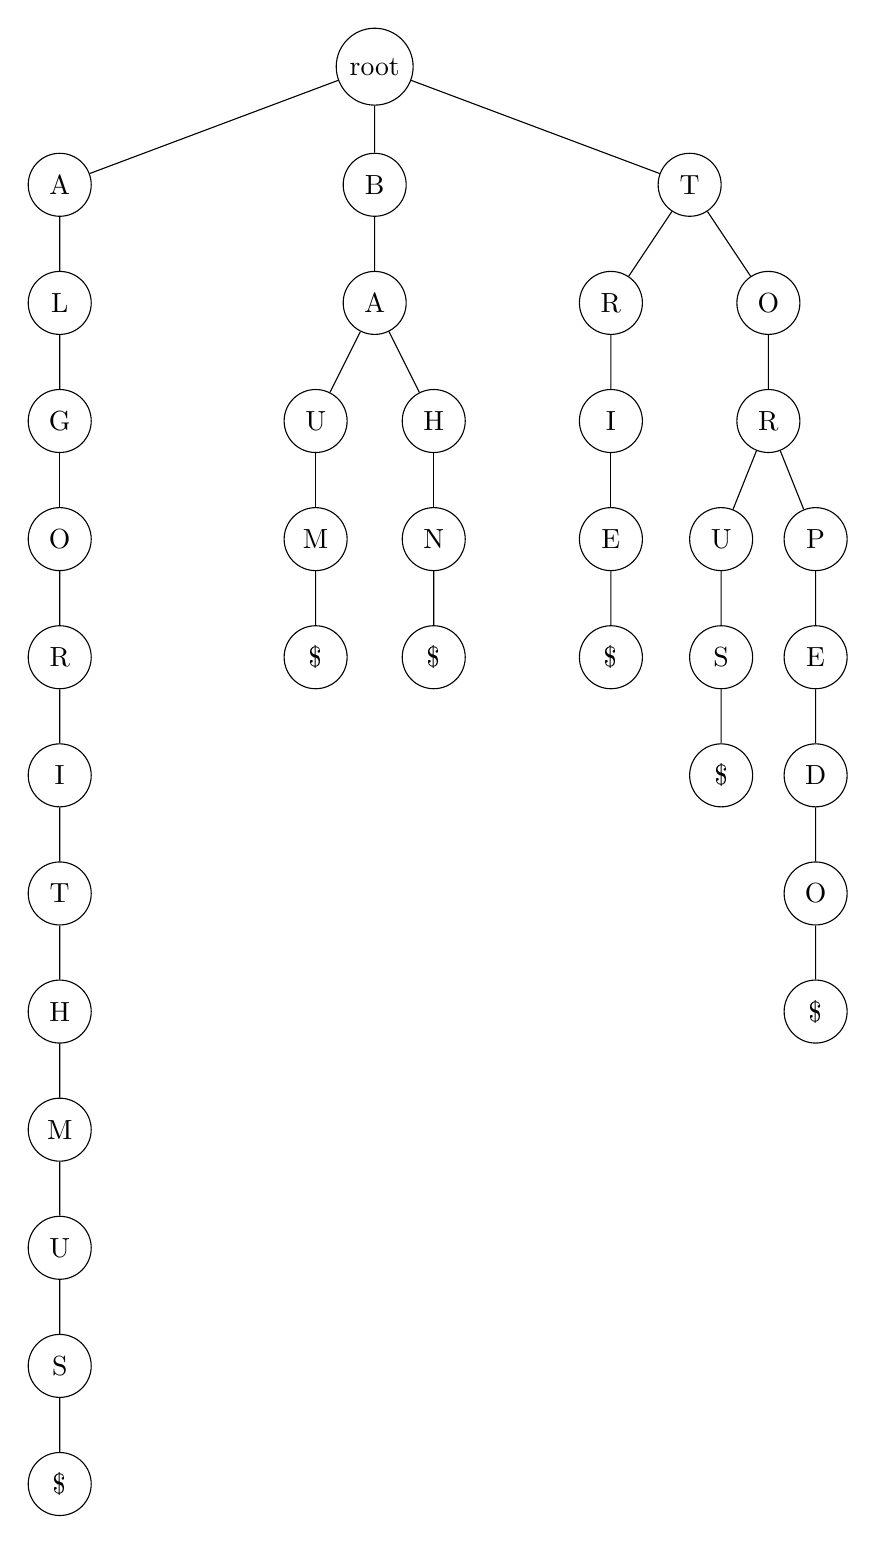
\begin{tikzpicture}[
  level distance=1.5cm,
  level 1/.style={sibling distance=4cm},
  level 2/.style={sibling distance=2cm},
  level 3/.style={sibling distance=1.5cm},
  level 4/.style={sibling distance=1.2cm},
  level 5/.style={sibling distance=1cm},
  every node/.style={draw, circle, minimum size=0.8cm}
]

\node {root}
  child {node {A}
    child {node {L}
      child {node {G}
        child {node {O}
          child {node {R}
            child {node {I}
              child {node {T}
                child {node {H}
                  child {node {M}
                    child {node {U}
                      child {node {S}
                        child {node {\$}}
                      }
                    }
                  }
                }
              }
            }
          }
        }
      }
    }
  }
  child {node {B}
    child {node {A}
      child {node {U}
        child {node {M}
          child {node {\$}}
        }
      }
      child {node {H}
        child {node {N}
          child {node {\$}}
        }
      }
    }
  }
  child {node {T}
    child {node {R}
      child {node {I}
        child {node {E}
          child {node {\$}}
        }
      }
    }
    child {node {O}
      child {node {R}
        child {node {U}
          child {node {S}
            child {node {\$}}
          }
        }
        child {node {P}
          child {node {E}
            child {node {D}
              child {node {O}
                child {node {\$}}
              }
            }
          }
        }
      }
    }
  };
\end{tikzpicture}

\newpage

\textbf{komprimierten Trie:}

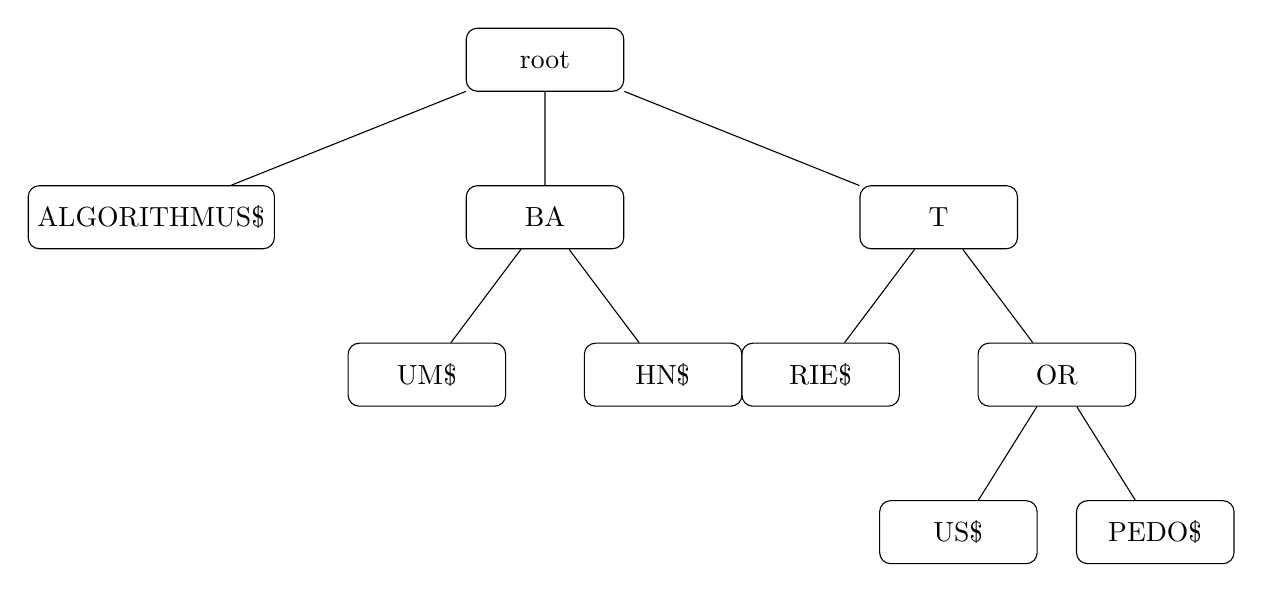
\begin{tikzpicture}[
  level distance=2cm,
  level 1/.style={sibling distance=5cm},
  level 2/.style={sibling distance=3cm},
  level 3/.style={sibling distance=2.5cm},
  every node/.style={draw, rectangle, rounded corners, minimum height=0.8cm, minimum width=2cm, align=center}
]

\node {root}
  child {node {ALGORITHMUS\$}}
  child {node {BA}
    child {node {UM\$}}
    child {node {HN\$}}
  }
  child {node {T}
    child {node {RIE\$}}
    child {node {OR}
      child {node {US\$}}
      child {node {PEDO\$}}
    }
  };
\end{tikzpicture}

\vspace{1cm}
\begin{center}
\small\textit{Enthält die Wörter: ALGORITHMUS, TRIE, BAUM, TORUS, BAHN, TORPEDO}
\end{center}





\noindent
\textbf{b)} Entwickeln Sie einen Algorithmus, der alle Wörter in einem unkomprimierten Trie ausgibt und dabei jede Kante höchstens zweimal besucht.\\


\section*{Algorithmus: Alle Wörter in einem Trie extrahieren}

\textbf{Beschreibung:}

Der folgende Algorithmus durchläuft einen gegebenen Trie rekursiv und sammelt alle vollständigen Wörter, die im Trie enthalten sind. Jede Kante des Trie wird dabei genau einmal besucht. Die Rekursion verzweigt sich immer dann, wenn mehrere mögliche Folgeknoten für einen Eintrag existieren.

\begin{enumerate}
    \item Übergabeparameter: \texttt{curr\_node = Trie.root}, \texttt{curr\_pr\"afix = ""}, \texttt{words = []}
    \item Wenn ein Eintrag des aktuell betrachteten Knotens das Stringende-Symbol (\texttt{*}) ist, dann stellt der Pfad von der Wurzel bis zu diesem Knoten ein vollständiges Wort dar.
    \begin{itemize}
        \item $\Rightarrow$ Füge dieses Wort zur Liste \texttt{words} hinzu.
    \end{itemize}
    \item Iteriere über alle Einträge \texttt{char} des aktuellen Knotens:
    \begin{itemize}
        \item Wenn der Eintrag \texttt{char} \emph{nicht} das Stringende-Symbol ist:
        \begin{itemize}
            \item $\Rightarrow$ Rufe die Funktion rekursiv auf mit: \\
            \texttt{curr\_node = curr\_node[char]}, \\
            \texttt{curr\_pr\"afix += char}, \\
            \texttt{words = words}
        \end{itemize}
    \end{itemize}
    \item Gib die Liste \texttt{words} zurück. Diese enthält nun alle Wörter, die im Trie gespeichert sind.
    \item Iteriere über die \texttt{words}-Liste und gebe jedes Wort aus.
\end{enumerate}

\newpage

\section*{Implementierung (Python)}

\begin{lstlisting}[language=Python]
class Trie:
    def __init__(self):
        self.root = {}
        self.end_symbol = "*"

    def add(self, word):
        current_level = self.root
        for letter in word:
            if letter not in current_level:
                current_level[letter] = {}
            current_level = current_level[letter]
        current_level[self.end_symbol] = True

    def search_level(self, current_level, current_prefix, words):
        if self.end_symbol in current_level:
            words.append(current_prefix)
        for letter in sorted(current_level.keys()):
            if letter != self.end_symbol:
                self.search_level(current_level[letter], current_prefix + letter, words)
        return words

    def words_with_prefix(self, prefix):
        collected_words = []
        current_level = self.root
        for letter in prefix:
            if letter not in current_level:
                return []
            current_level = current_level[letter]
        return self.search_level(current_level, prefix, collected_words)


def main():
    trie = Trie()
    trie.add("help")
    trie.add("hello")
    trie.add("hi")
    found_words = trie.search_level(trie.root,"",[])
    for word in found_words:
        print(word)

main()
\end{lstlisting}

\subsection*{Ausgabe:}
\begin{verbatim}
hello
help
hi
\end{verbatim}

\subsection*{Anmerkung:}

Der Funktionsaufruf \texttt{trie.search\_level(trie.root, "", [])} zusammen mit dem anschließenden \texttt{print}-Block implementiert exakt den oben beschriebenen Algorithmus. Der Rekursionsbaum verzweigt sich bei jedem Knoten mit mehreren Kindknoten. Jede Kante im Trie wird dabei genau einmal besucht.